\documentclass{article}
    \usepackage[utf8]{inputenc}
    \usepackage{graphicx}
    \title{Trabalho Final \\ Biblioteca}
    \author{ Alex Raimundo de Oliveira \\ Victor Geraldo Faria Costa\\ Yuri Dimitre Dias de Faria}
    \date{Setembro 2021}
    
  
    
    \begin{document}
    
    \maketitle
\section*{O Diagrama Entidade Relacionamento (DER):}
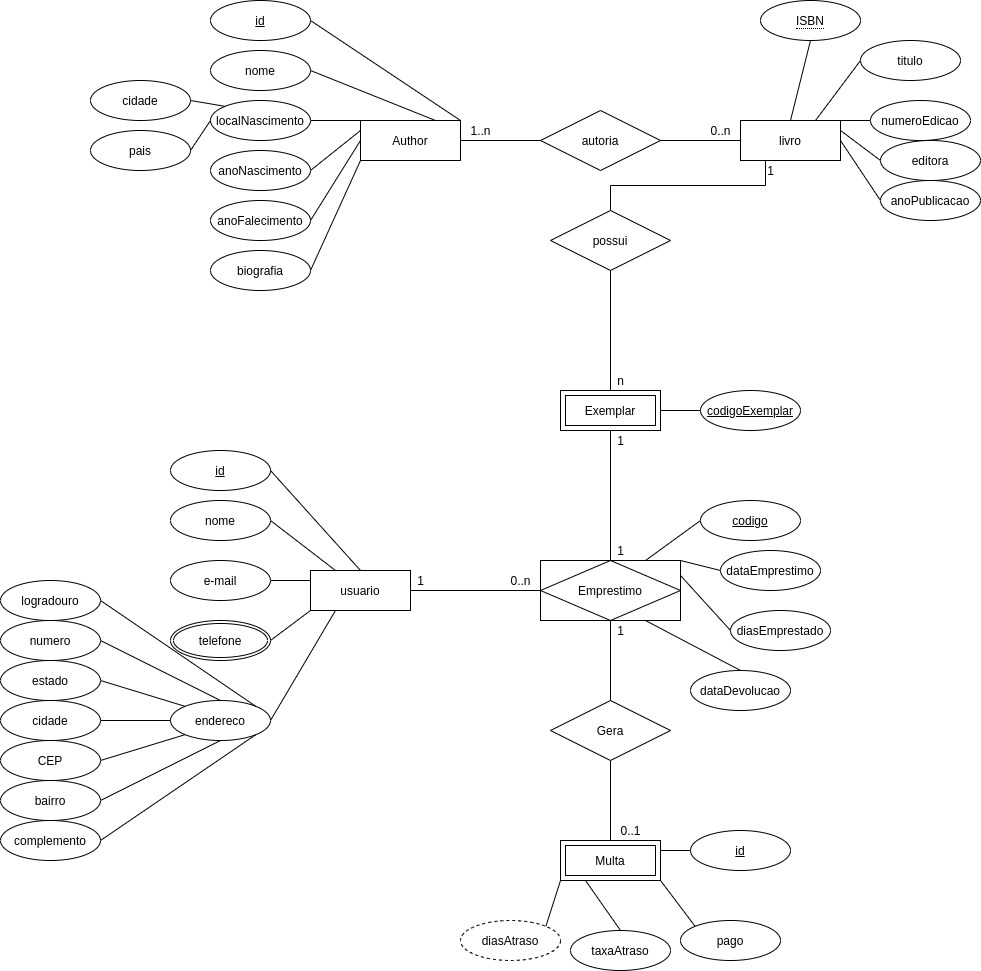
\includegraphics[height=\hsize]{../docs/DER2.png}
\section*{Diagrama de Tabelas Relacionais}
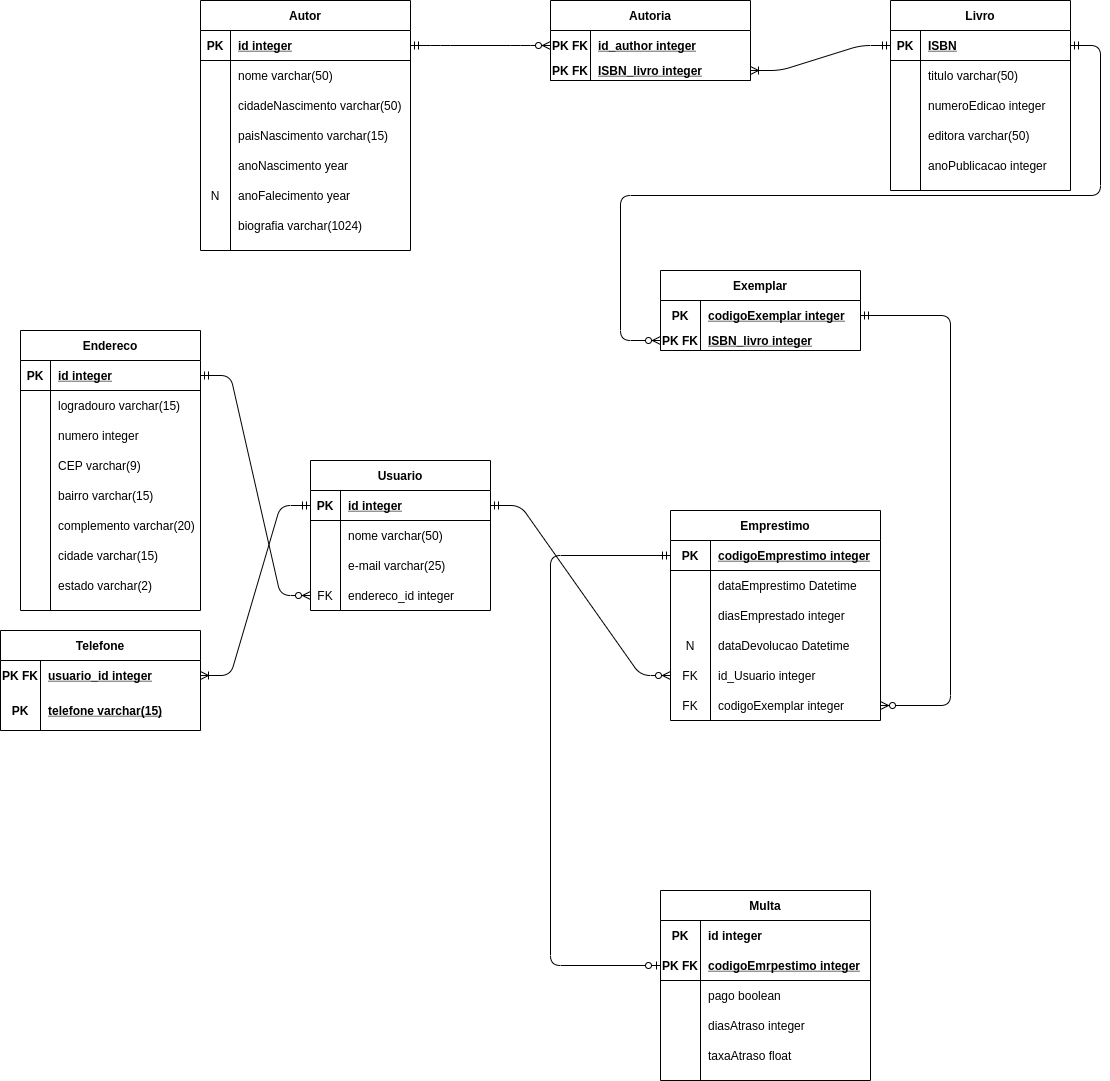
\includegraphics[height=\hsize]{../docs/MR.png}
\begin{itemize}
    \item Foi utilizado uma tabela separada para armazenamento de endereços para ser possível dois ou mais usuários possuírem endereço em comum.
    \item A tabela telefone foi criada de forma desacoplada do usuário para permitir múltiplos telefones, já que é um campo multivalorado
    \item A tabela autoria foi criada para que seja possível um livro possuir mais de um autor.
\end{itemize} 
  
    \end{document}
    